% Nallino, Part I p. 90: the figure of the new Moon, redrawn from the print: the disc of the Sun ABCD
% (centre E) and the equal disc of the Moon (centre F), the diameters AC and BD, the line MS, the
% line HK produced to L, the line through F, E and G to T, and the line PQ through the intersections
% of the discs; the four quarters MERIDIES, ORIENS, OCCIDENS, SEPTENTRIONES (the first N of the last
% printed reversed). Circles and lines are least-squares fits to the printed ink; coordinates are
% PDF points of master page 179 less the origin (95.04, 108.06), y downward.
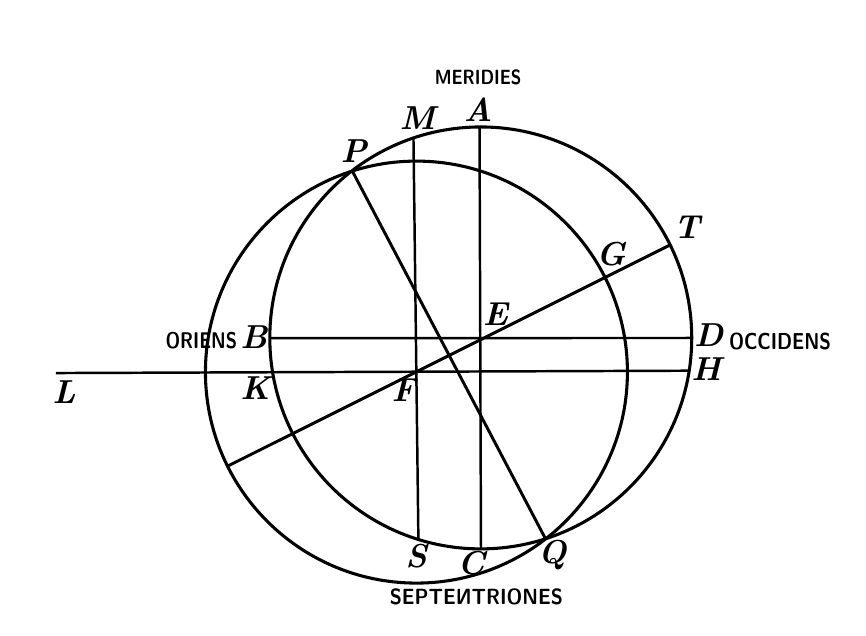
\begin{tikzpicture}[x=0.9894pt,y=-0.9894pt,line cap=butt,every node/.style={font=\fontsize{11.5}{11.5}\bfseries\itshape\selectfont,inner sep=0pt}]
\useasboundingbox (0,0) rectangle (296.00,212.00);
\draw[line width=1.11pt] (165.48,113.31) circle[radius=77.05];  % the disc of the Sun ABCD, centre E
\draw[line width=1.11pt] (141.98,125.79) circle[radius=77.06];  % the disc of the Moon, centre F (equal to the disc of the Sun)
\draw[line width=0.89pt] (165.02,36.26) -- (165.56,190.36);  % the diameter AC through E
\draw[line width=0.89pt] (88.43,113.38) -- (242.53,113.33);  % the diameter BD through E (the line of the ecliptic)
\draw[line width=0.89pt] (140.90,40.29) -- (142.70,186.92);  % the line MS (the arcs AM and CS equal to the distance of Sun and Moon)
\draw[line width=0.89pt] (10.27,126.14) -- (241.59,125.28);  % the line HK produced to L (KL equal to EB)
\draw[line width=1.06pt] (73.00,160.16) -- (234.64,79.35);  % the line through F and E to T (G where it leaves the disc of the Moon)
\draw[line width=1.06pt] (118.50,52.24) -- (189.11,186.65);  % the line PQ through the intersections of the two discs
\node at (142.34,33.10) {M};
\node at (164.46,30.04) {A};
\node at (119.11,45.19) {P};
\node at (240.72,72.77) {T};
\node at (213.06,82.74) {G};
\node at (170.81,104.68) {E};
\node at (82.65,112.89) {B};
\node at (248.73,112.18) {D};
\node at (247.86,124.74) {H};
\node at (13.22,133.03) {L};
\node at (83.09,131.77) {K};
\node at (137.29,132.55) {F};
\node at (141.92,193.08) {S};
\node at (161.96,195.54) {C};
\node at (191.63,192.57) {Q};
\node at (164.52,18.31) {\normalfont\fontsize{8.5}{8.5}\sffamily\bfseries\selectfont \resizebox{31.25pt}{5.16pt}{MERIDIES}};
\node at (63.41,114.40) {\normalfont\fontsize{8.5}{8.5}\sffamily\bfseries\selectfont \resizebox{25.82pt}{5.70pt}{ORIENS}};
\node at (274.78,114.44) {\normalfont\fontsize{8.5}{8.5}\sffamily\bfseries\selectfont \resizebox{36.86pt}{5.79pt}{OCCIDENS}};
\node at (163.88,207.86) {\normalfont\fontsize{8.5}{8.5}\sffamily\bfseries\selectfont \resizebox{62.51pt}{5.52pt}{SEPTE\reflectbox{N}TRIONES}};
\end{tikzpicture}
